Die Produktfunktionen beschreiben jede einzelne Funktion des Produkts mittels Anwendungsfalldiagrammen und Anwendungsfalltabellen.
\\\\
In  Tabelle~\autoref{fig:akteur-tabelle} werden alle auftretenden Akteure beschrieben.


\begin{figure}[h]
	\centering
	
	\begin{tabularx}{\textwidth}{ p{.1\textwidth} | p{.4\textwidth} | X }
		\textbf{Akteur} & \textbf{Beschreibung} & \textbf{Verwendet in Anwendungsszenario} \\ \hline
		NutzerIn & Nutzt den SWARM Composer & APP-1, APP-2, APP-3, APP-4
		\\ \hline AdministratorIn & Nutzt und verwaltet den SWARM-Composer & APP-1, APP-2, APP-3, APP-4
	\end{tabularx}
	
	\caption{Beschreibung der Akteure}
	\label{fig:akteur-tabelle}
\end{figure}


%%%%%%%%%%%%%%%
%% Anwendungsfall 1 %%
%%%%%%%%%%%%%%%
\newpage

\section{Anwendungsfalldiagramm - App}

\begin{figure}[h]
	\centering	
	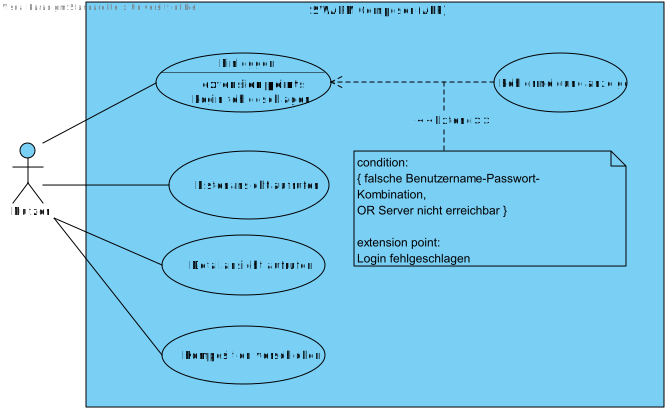
\includegraphics[width=\textwidth]{img/Produktfunktionen_app}	
	\caption{Anwendungsfalldiagramm - App}
	\label{fig:anwendungsfalldiagramm-app}
\end{figure}

\newpage

\begin{figure}[h]
	\centering
	\begin{tabularx}{\textwidth}{ X | X }
		\textbf{Anwendungsfall ID} & APP-1 \\ \hline
		\textbf{Anwendungsfallname} & Einloggen \\ \hline
		\textbf{Initiierender Akteur} & NutzerIn \\ \hline
		\textbf{Weitere Akteure} & -  \\ \hline
		\textbf{Kurzbeschreibung} & Der Nutzer loggt sich ein.  \\ \hline
		\textbf{Vorbedingungen} & Die Android-App ist geöffnet. Der Nutzer ist nicht eingeloggt.  \\ \hline
		\textbf{Nachbedingungen} & Der Nutzer ist eingeloggt.  \\ \hline
		\textbf{Ablauf} &
			\begin{enumerate}
				\item Der Nutzer gibt seinen Benutzernamen ein.
				\item Der Nutzer gibt sein Passwort ein.
				\item Der Nutzer tippt auf den Login-Button.
				\item Eine Bestätigung der erfolgreichen Anmeldung wird angezeigt.
			\end{enumerate} \\ \hline
		\textbf{Alternative} &
				- \\ \hline
		\textbf{Ausnahme} &
				\begin{enumerate}
					\item Der Nutzer gibt seinen Benutzernamen ein.
					\item Der Nutzer gibt sein Passwort ein.
					\item Der Nutzer tippt auf den Login-Button.
					\item Die Anmeldung schlägt fehl und eine Fehlermeldung wird angezeigt.
				\end{enumerate}  \\ \hline
		\textbf{Benutzte Anwendungsfälle} & Fehlermeldung anzeigen \\ \hline
		\textbf{Spezielle Anforderungen} & - \\ \hline
		\textbf{Annahmen} & -
	\end{tabularx}
	\caption{Anwendungsfall APP-1}
	\label{fig:anwendungsfall-app-tabelle-APP-1}
\end{figure}

\newpage

\begin{figure}[h]
	\centering
	\begin{tabularx}{\textwidth}{ X | X }
		\textbf{Anwendungsfall ID} & APP-2 \\ \hline
		\textbf{Anwendungsfallname} & Listenansicht aufrufen \\ \hline
		\textbf{Initiierender Akteur} & NutzerIn \\ \hline
		\textbf{Weitere Akteure} & -  \\ \hline
		\textbf{Kurzbeschreibung} & Dem Nutzer wird eine Liste von vorhandenen Kompositionen angezeigt.  \\ \hline
		\textbf{Vorbedingungen} & Die App ist geöffnet.  \\ \hline
		\textbf{Nachbedingungen} & Dem Nutzer wird eine Liste von vorhandenen Kompositionen angezeigt.  \\ \hline
		\textbf{Ablauf} &
		\begin{enumerate}
			\item Die für den Nutzer sichtbaren Kompositionen werden vom Server abgerufen.
			\item Die Daten werden als Liste angezeigt.
		\end{enumerate} \\ \hline
		\textbf{Alternative} &
		\begin{enumerate}
			\item Der Nutzer kehrt zur Listenansicht zurück.
			\item Ihm wird eine Liste der für ihn sichtbaren Kompositionen angezeigt.
		\end{enumerate}  \\ \hline
		\textbf{Ausnahme} &
		-  \\ \hline
		\textbf{Benutzte Anwendungsfälle} & - \\ \hline
		\textbf{Spezielle Anforderungen} & - \\ \hline
		\textbf{Annahmen} & -
	\end{tabularx}
	\caption{Anwendungsfall APP-2}
	\label{fig:anwendungsfall-app-tabelle-APP-2}
\end{figure}

\newpage

\begin{figure}[h]
	\centering
	\begin{tabularx}{\textwidth}{ X | X }
		\textbf{Anwendungsfall ID} & APP-3 \\ \hline
		\textbf{Anwendungsfallname} & Detailansicht aufrufen \\ \hline
		\textbf{Initiierender Akteur} & NutzerIn \\ \hline
		\textbf{Weitere Akteure} & -  \\ \hline
		\textbf{Kurzbeschreibung} & Der Nutzer ruft die Detailansicht einer Komposition auf.  \\ \hline
		\textbf{Vorbedingungen} & Der Nutzer hat die Listenansicht aufgerufen.  \\ \hline
		\textbf{Nachbedingungen} & Dem Nutzer wird die Detailansicht einer Komposition gezeigt.  \\ \hline
		\textbf{Ablauf} &
		\begin{enumerate}
			\item Der Nutzer wählt in der Listenansicht eine Komposition aus.
			\item Dem Nutzer werden die Details der ausgewählten Komposition angezeigt.
		\end{enumerate} \\ \hline
		\textbf{Alternative} &
		-  \\ \hline
		\textbf{Ausnahme} &
		- \\ \hline
		\textbf{Benutzte Anwendungsfälle} & - \\ \hline
		\textbf{Spezielle Anforderungen} & - \\ \hline
		\textbf{Annahmen} & -
	\end{tabularx}
	\caption{Anwendungsfall APP-3}
	\label{fig:anwendungsfall-app-tabelle-APP-3}
\end{figure}

\newpage

\begin{figure}[h]
	\centering
	\begin{tabularx}{\textwidth}{ X | X }
		\textbf{Anwendungsfall ID} & APP-4 \\ \hline
		\textbf{Anwendungsfallname} & Komposition verschicken \\ \hline
		\textbf{Initiierender Akteur} & Nutzer \\ \hline
		\textbf{Weitere Akteure} & -  \\ \hline
		\textbf{Kurzbeschreibung} & Der Nutzer verschickt eine Komposition.  \\ \hline
		\textbf{Vorbedingungen} & Der Nutzer hat in der Listenansicht eine Komposition ausgewählt und die Detailansicht aufgerufen.  \\ \hline
		\textbf{Nachbedingungen} & Die Komposition wird verschickt.  \\ \hline
		\textbf{Ablauf} &
		\begin{enumerate}
			\item Dem Nutzer wird eine Komposition in der Detailansicht angezeigt.
			\item Der Nutzer tippt auf den Verschicken-Button.
			\item Eine Datei im PDF-Format wird erstellt.
			\item Der Nutzer bestätigt den Versand.
		\end{enumerate} \\ \hline
		\textbf{Alternative} &
		-  \\ \hline
		\textbf{Ausnahme} &
		- \\ \hline
		\textbf{Benutzte Anwendungsfälle} & - \\ \hline
		\textbf{Spezielle Anforderungen} & - \\ \hline
		\textbf{Annahmen} & -
	\end{tabularx}
	\caption{Anwendungsfall APP-4}
	\label{fig:anwendungsfall-app-tabelle-APP-4}
\end{figure}

\newpage

%%%%%%%%%%%%%%%
%% Anwendungsfall 2 %%
%%%%%%%%%%%%%%%

\section{Anwendungsfalldiagramm - Server}

\begin{figure}[h]
	\centering
	\missingfigure{Anwendungsfalldiagramm - Server}		
	\caption{Anwendungsfalldiagramm - Server}
	\label{fig:anwendungsfalldiagramm-server}
\end{figure}

\newpage

\begin{figure}[h]
	\centering
	\begin{tabularx}{\textwidth}{ X | X }
		\textbf{Anwendungsfall ID} & XX-1 \\ \hline
		\textbf{Anwendungsfallname} & Hier steht ein Name. \\ \hline
		\textbf{Initiierender Akteur} & Informatiker \\ \hline
		\textbf{Weitere Akteure} & Designer, Techniker  \\ \hline
		\textbf{Kurzbeschreibung} & Hier steht eine Kurzbeschreibung.  \\ \hline
		\textbf{Vorbedingungen} & -  \\ \hline
		\textbf{Nachbedingungen} & Y trifft zu.  \\ \hline
		\textbf{Ablauf} &
		\begin{enumerate}
			\item Erster ganzer Satz.
			\item Zweiter ganzer Satz.
		\end{enumerate} \\ \hline
		\textbf{Alternative} &
		\begin{enumerate}
			\item Erster ganzer Satz.
			\item Zweiter ganzer Satz.
		\end{enumerate}  \\ \hline
		\textbf{Ausnahme} &
		\begin{enumerate}
			\item Erster ganzer Satz.
			\item Zweiter ganzer Satz.
		\end{enumerate}  \\ \hline
		\textbf{Benutzte Anwendungsfälle} & YY-1 (oder Name) \\ \hline
		\textbf{Spezielle Anforderungen} & - \\ \hline
		\textbf{Annahmen} & -
	\end{tabularx}
	\caption{Anwendungsfall XX-1}
	\label{fig:anwendungsfall-server-tabelle-xx-1}
\end{figure}